\documentclass[letterpaper,10pt]{article}
\usepackage{graphicx}
\usepackage[export]{adjustbox}
\usepackage{fancyhdr}
\usepackage[spanish]{babel}
\usepackage{listings}
\usepackage[utf8]{inputenc}
\pagenumbering{roman}
\usepackage[left=2.5cm,
top=2.5cm,
right=2.5cm,
bottom=3cm]{geometry}
\usepackage{listings}
%\pagenumbering{gobble}
\usepackage{ragged2e} 
%\usepackage{fancy}
\usepackage{placeins}
\pagestyle{fancy}
\fancyhf{}
\usepackage[spanish]{babel}
\usepackage[utf8]{inputenc}
\usepackage[left=2.5cm,
top=2.5cm,
right=2.5cm,
bottom=3cm]{geometry}
\begin{document}
	
\begin{titlepage}
	
	\begin{center}
		\vspace*{-1in}
		\begin{figure}[htb]
			\centering
			
\includegraphics[scale=1.5]{ESCUDO}
		\end{figure}
		
		\textbf{TECNOLÓGICO NACIONAL DE MÉXICO}\\
		\vspace*{0.15in}
		INSTITUTO TECNOLÓGICO DE MORELIA \\
		\vspace*{0.3in}
		\begin{large}
			DEPARTAMENTO DE INGENIERÍA ELECTRÓNICA\\
		\end{large}
		\vspace*{0.2in}
		\begin{large}
			CONTROL I\\
		\end{large}
		\vspace*{0.3in}
		\begin{Large}
			\textbf{PRACTICA DE LABORATORIO No.1: \\
			Analysis of a first order system}\\ 
		\end{Large}
		\vspace*{0.3in}
		\begin{large}
		\textbf{PROFESOR:} GERARDO MARX CHÁVEZ CAMPOS\\
		\end{large}
		\vspace*{0.2in}
		\begin{large}
			JESÚS ANTONIO MAGAÑA SILVA: \textbf{14121126}\\
			VÍCTOR HUGO GARCÍA VALDIVIA: \textbf{14121088}
		\end{large}
		\vspace*{0.3in}
		\rule{80mm}{0.1mm}\\
		\vspace*{0.1in}
		\begin{large}
			MORELIA, MICHOACÁN \\
			OCTUBRE, 2017 \\
		\end{large}
	\end{center}
\end{titlepage}


	\pagebreak
	\justify
	\tableofcontents
	\pagebreak
	\pagenumbering{arabic}
	\section{Introducción}
	\vspace*{0.3in}
	El objetivo de la práctica es comenzar a familiarizarse con el software matemático Scilab o en su defecto Matlab, tanto para realizar cálculos como para gráficar. En este caso se utilizó para saber la respuesta de un sistema eléctrico  equivalente a nuestro sistema hidráulico en respuesta de la frecuencia o en tiempo para generar la gráfica del sistema y/o comportamiento del mismo.
	
	%Figura\ref{fig: Foto 2}
	\begin{figure}[h!]
		\centering
		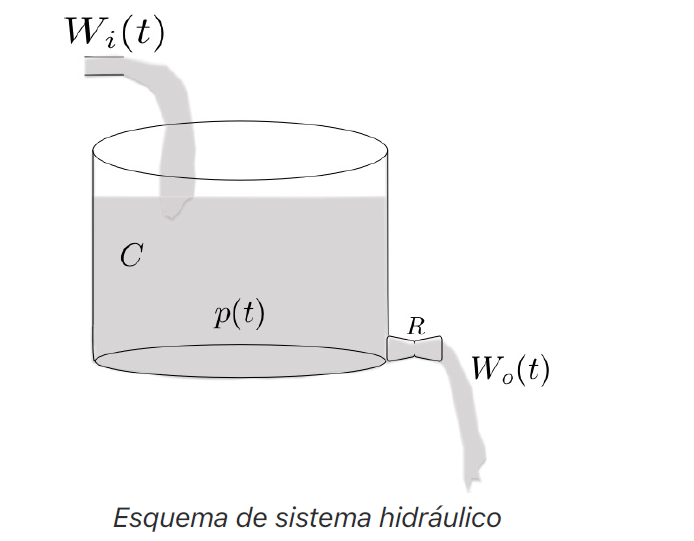
\includegraphics[scale=0.85]{hidraulico}
		\caption{Esquema de sistema hidraulico}
	%	\label{fig: Foto 2}
	\end{figure}
	
	\vspace*{0.3in}
	Y una vez sacando la función de transferencia con respecto a tiempo (usando la transformada inversa de Laplace), se implemtara un código para que en el mismo software se puedan ingresar los valores de cualquier sistema que sea de primer orden y facilitar su procesamiento.
	
	\pagebreak
    \section{Metodología}
    %\begin{itemize}
    \vspace*{0.3in}
    	Realizar un análisis del circuito equivalente eléctrico resultante del circuito hidráulico, tomando en cuenta el equivalente de la corriente de entrada y el de la corriente de salida mostrando las corrientes de cada elemnto con el análisis de corrientes de kirkchoff. 
    %\end{itemize}
    
    %	Figura\ref{fig: Foto 1}
    \vspace*{0.3in}
    	\begin{figure}[h!]
    		\centering
    		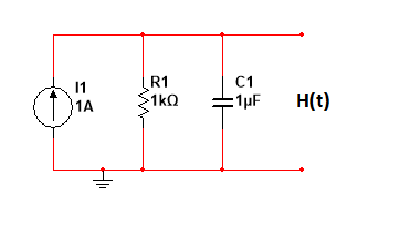
\includegraphics[scale=1.2]{circuito1.png}
    		\caption{Diagrama del Circuito}
    %		\label{fig: Foto 1}
    	\end{figure}
    
    \vspace*{0.3in}
    \begin{equation}
    W_i(t) = \frac {h(t)}{R} + \frac {Cdh(t)}{dt}\\
    \end{equation}
        \begin{equation}    
    W_i(S) = \frac {H(S)}{R} + CSH(S)+H(0)\\
    \end{equation}
        \begin{equation}
    W_i(S) = H(S)(\frac{1}{R} + CS)
    \end{equation}
    \begin{equation}    
    G(S) = \frac{W_i(S)}{H(S)}
    \end{equation}
    \begin{equation}
    G(S) = H(S)(\frac{1}{\frac{1}{R} + CS})
    \end{equation}
	\begin{equation}
	W_i(S) = H(S)(\frac{1}{R} + CS)
	\end{equation}
	 \begin{equation}
	G(S) = H(S)(\frac{1}{C\frac{1}{RC} + CS}) = \frac{\frac{1}{c}}{s+\frac{1}{RC}}
	\end{equation}
    
\pagebreak
 \begin{equation}
Y(t) = (\frac{1}{c})exp^\frac{-t}{RC}
\end{equation}
 \begin{equation}
Y(t) = \frac{c}{a}+(b-\frac{c}{a}){exp^-at}
\end{equation}

\vspace*{0.3in}
\textbf{}
 Mediante las ecuaciones anteriores sacamos la transformada inversa de Laplace,
 desde la funcion de tranferencia de un sistema de energía de primer orden (8) lo cual la se dejó en términos variables para (9) para facilitar el análisis de cualquier sistema de energía de primer orden. 
 
 \pagebreak
 
 \section{Código}
\begin{center}
	\begin{lstlisting}[frame=single]
	
	a=input('a=');
	b=input('b=');
	c=input('c=');
	t=0:0.01:15;
	Function_t=(c/a)+(b-(c/a))*exp(-a*t);
	plot(t,Function_t,'r')
	title('Funcion de Transferencia');
	xlabel('segundos(s)','FontSize', 16);
	ylabel('funcion','FontSize', 16); 
	\end{lstlisting}
\end{center}
\FloatBarrier


\vspace*{0.3in}
\textbf{}
Gracias al código anterior se pueden mostrar las graficas siguientes donde se tomara en cuenta las siguientes condiciones:\\ $ Wi = Wo $ (El nivel permanece constante)\\$ Wi > Wo $ (El nivel se eleva)\\$ Wi < Wo $ (El nivel decae)\\

%\vspace*{0.5in}
%\begin{itemize}[here!]
%\item Wi = Wo
%\end{itemize}

    %	Figura\ref{fig: Foto 1}
\vspace*{0.3in}
\begin{figure}[h!]
	\begin{itemize}
		\item $ Wi = Wo $
	\end{itemize}
	\centering
	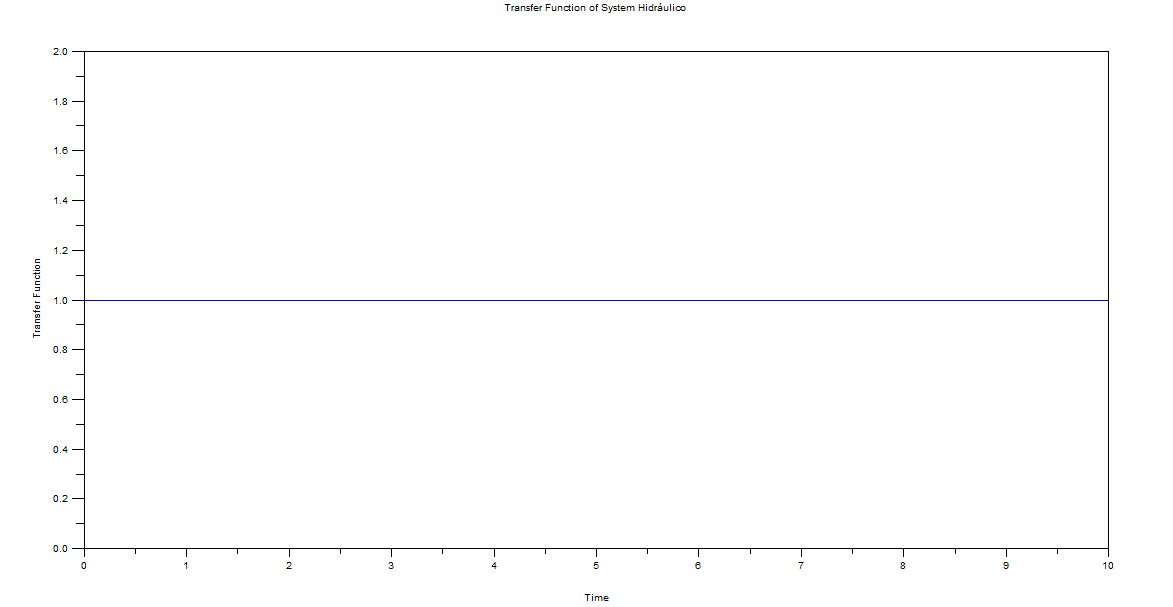
\includegraphics[scale=0.3]{constante}
	\caption{Gráfica de carga constante $ Wi = Wo $}
	%		\label{fig: Foto 1}
\end{figure}


    %	Figura\ref{fig: Foto 1}
\vspace*{0.3in}
\begin{figure}[h!]
	\begin{itemize}
		\item $ Wi > Wo $
	\end{itemize}
	\centering
	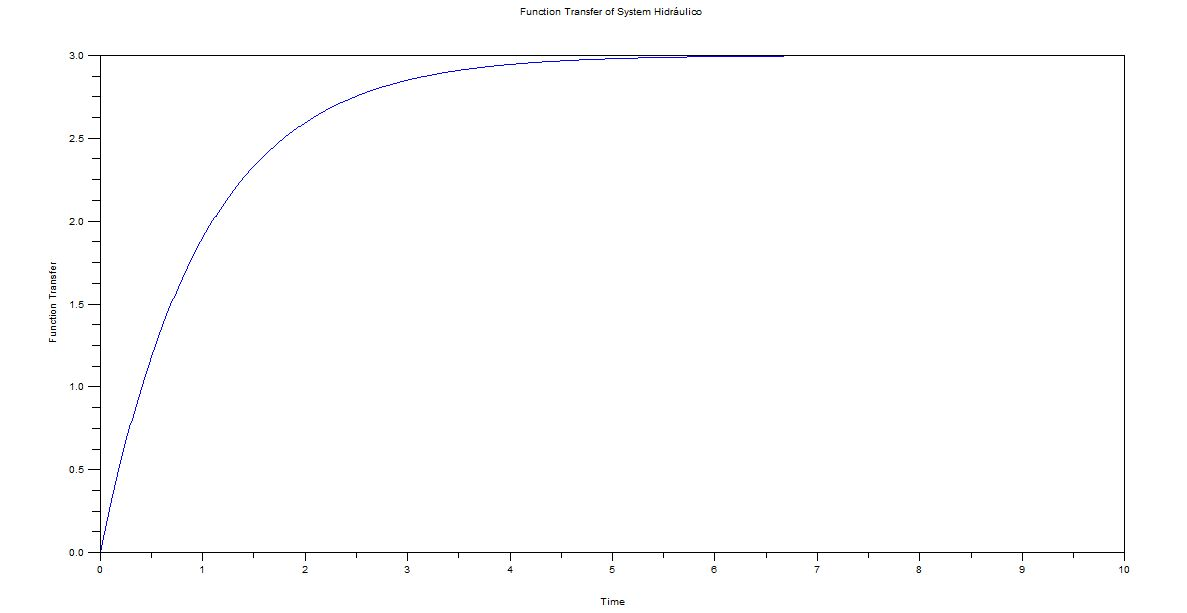
\includegraphics[scale=0.3]{carga}
	\caption{Gráfica del capactor cargandose $ Wi > Wo $}
	%		\label{fig: Foto 1}
\end{figure}

    %	Figura\ref{fig: Foto 1}
\vspace*{0.3in}
\begin{figure}[h!]
	\begin{itemize}
		\item $ Wi < Wo $
	\end{itemize}
	\centering
	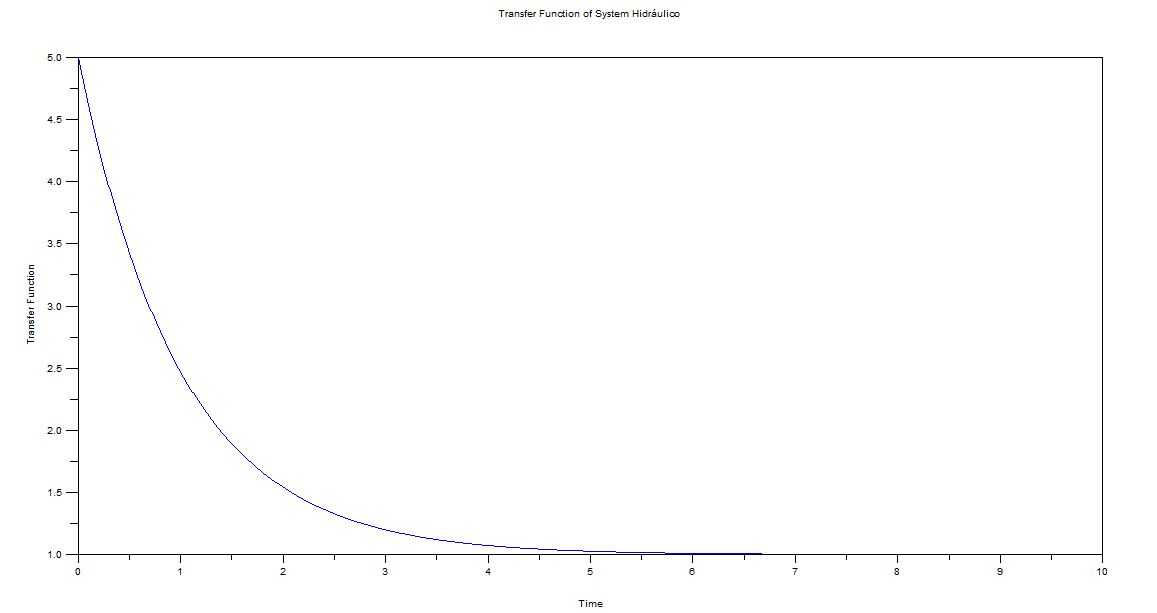
\includegraphics[scale=0.3]{descarga}
	\caption{Gráfica de descarga del capacitor $ Wi < Wo $}
	%		\label{fig: Foto 1}
\end{figure}

\newpage
\vspace*{1.5in}

\section{Conclusiones}
\vspace*{0.3in}
\textbf{Victor Hugo Garcia valdivia\\}
En la práctica no encontramos con unos problemas de compatibilidad usando el software Scilab.
Pero concluyo en que en esta practica podemos hacer programas enfocados a la resolución u 
obtención de la Función de Transferencia en respuesta con el tiempo para ver cómo se comporta
un sistema de primer orden. En este caso se implementó la solucion general de un sistema de 
primer orden sacando la Funcion de transferencia mediante la Transformada inversa de Laplace y
obteniendola en función del tiempo.\\
	 
\vspace*{0.3in}
	  
\textbf{Jesús Antonio Magaña Silva} \\
Concluir que durante esta practica toda la teoría antes vista en clase sobre la funcion de transferencia de primer orden y sacar el equivale de un circuito hidraulico a uno electrico mostrando sus equivalencias de componentes fue llevada a cabo de manera practica con un problema real, así como la funcion de tranferencia de dicho diagrama comprobando en esta práctica la de carga y descarga de un capacitor siendo el equivalente del recipiente contenedor de agua, asi como las funciones con que cuenta el software Scilab y Matlab\\
\end{document}